\documentclass[12pt, a4paper]{article}
\usepackage{amsmath}
\usepackage{amsfonts}
\usepackage{amsthm}
\usepackage{mathtools}
\newtheorem{theorem}{Theorem}[section]
\newtheorem{definition}{Definition}[section]
\numberwithin{equation}{section}
\usepackage{pgfplots}
\pgfplotsset{width=10cm,compat=1.9}
\graphicspath{ {img/} }
\DeclareGraphicsExtensions{.png}

\title{Reinforcement Learning}
\author{Kristian Wichmann}

\begin{document}
\maketitle

\section{Basics of reinforcement learning}
\textit{Reinforcement learning} deals with an \textit{agent} making \textit{decisions} over time in dealing with some \textit{environment}, to maximize some cumulative, scalar \textit{reward}.

An example would be playing a video game. Here, the player is the agent. The control inputs are the decisions. The game and its internal logic is the environment. And the score is the reward.

Sometimes, a reward will be greater if it is postponed - it is not always advantagegous to reap any immediate reward. In other words, reinforcement learning algorithms will not benefit from being greedy.

\subsection{The reward hypothesis}
The basis of all reinforcement learning is the \textit{reward hypothesis}, which states:

\begin{quotation}
All goals can be described by the maximization of some cumulative, expected reward.
\end{quotation}

\subsection{Observation, action, and reward}
At at given timestep $t$, a reinforcement learning agent gets some input; an \textit{observation} $O_t$ about the environment. It then takes an \textit{action} $A_t$. And finally it gets a scalar \textit{reward} $R_t$.

\begin{figure}
\centering
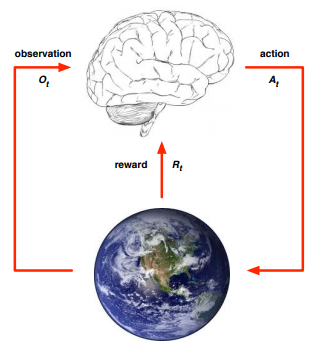
\includegraphics[width=0.6\textwidth]{agent_environment}
\caption{The interplay between agent and environment.}
\label{fig:agent_environment}
\end{figure}

\subsection{History and state}
At any given time step $t$, the agent has a \textit{history} $H_t$, which simply consist of all the observations, actions, and rewards that have happened so far:
\begin{equation}
H_t=O_1,A_1,R_1,O_2,A_2,R_2,\cdots,O_t,A_t,R_t,
\end{equation}
A \textit{state} is a way for to parse this history into a more meaningful form. Formally, the state representation is simply a function of the history:
\begin{equation}
S_t=f(H_t)
\end{equation}

It is very important to note, that this is generally distinct from the \textit{environment state} $H^e_t$. The environment state contains complete information about the environment, including data and mechanisms that may be hidden to the agent. Hence $H^e_t$ can depend on other things than just the historySuch information is \textit{private} to the environment.

The \textit{agent state} $S^a_t$ on the other hand is the internal representation the agent uses to decide on which actions to take. Once again, it can be any function of history:
\begin{equation}
S^a_t=f(H_t)
\end{equation}

\subsection{Markov states}
A state $S_{t+1}$ is called a \textit{Markov state} or an \textit{information state} if it only depends on the state of the previous time step. Expressed probabilistically:
\begin{equation}
\mathbb{P}[S_{t+1}|S_1,S_2,\cdots S_t]=\mathbb{P}[S_{t+1}|S_t]
\end{equation}
In other words, we don't need the entire history to decide on an action: Knowing the present is enough. Or put another way:
\begin{quotation}
The future is independent of the past, given the present.
\end{quotation}
Or:
\begin{quotation}
The state is a \textit{sufficient statistic} of the future.
\end{quotation}

The environment state is always Markov, as by definition it contains all information about what can happen next. Similarly, the state consisting of the entire history is trivially Markov as well.

\subsection{Full observability}
This is the case where, in fact, we can observe everything about the environment and its inner workings. So that:
\begin{equation}
O_t=S^a_t=S^e_t
\end{equation}
Sometimes this is reasonable. Sometimes not. But it will be a useful theoretical situation. This is known as a \textit{Markov decision process} or MDP for short.

When this condition is not fulfilled, we speak about \textit{partial observability} or a \textit{partially observable evironment}. Here the agent only indirectly observes the invironment. This situation is known as a \textit{partially observable Markov decision process} or POMDP for short.

\subsection{State example: Bayesian beliefs}
This state representation can be seen as a current best bet at what the actual environment state is. In other words, it is represented by Bayesian probabilities, which may then be updated over time using Bayes' rule:
\begin{equation}
S^a_t=(\mathbb{P}[S^e_t=s_1],\mathbb{P}[S^e_t=s_2],\cdots,\mathbb{P}[S^e_t=s_n])
\end{equation}

\subsection{State example: Recurrent neural net}
Here, the state $S^a_t$ is a linear combination of the observation $O_t$ and the state of the last time step $S^a_{t-1}$, followed by a non-linear \textit{activation function} $\sigma$:
\begin{equation}
S^a_t=\sigma(W_O O_t+W_S S^a_{t-1})
\end{equation}
Here, the $W$'s are weight matrices with sizes corresponding to the dimenstionality of observations and state vectors. Typical choices for $\sigma$ are sigmoid, tanh, or rectified linear unit.

\section{Components of an agent}
A reinforcement learning agent may contain one or more of the following components:
\begin{itemize}
\item \textit{Policy}: The agent's behaviour function. Shows how the agent gets from its state to deciding on an action.
\item \textit{Value function}: A measure of how desirable it is to be in a given state, or perform a given action.
\item \textit{Model}: The agent's representation of the environment.
\end{itemize}
We'll examine each of these in greater detail below:

\subsection{Policy}
A policy $\pi$ is a mapping from state to action. For a \textit{deterministic} policy, this is an ordinary function:
\begin{equation}
\pi(s)=a
\end{equation}
So the state $s$ is always mapped to the action $a$. We should ideal choose $\pi$ so that the reward is maximized. 

But a policy can also be \textit{stochastic}, i.e. probabilistic. In this case $\pi$ takes the form of conditional probabilities:
\begin{equation}
\pi(a|s)=\mathbb{P}[A=a|S=s]
\end{equation}

\subsection{Value function}
A value function $V_\pi$ is a prediction of the future reward for state $s$ under a given policy $\pi$:
\begin{equation}
V_\pi(s)=\mathbb{E}_\pi[R_t+\gamma R_{t+1}+\gamma^2 R_{t+2}+\cdots|S_t=s]
\end{equation}
Here $\gamma$ is a \textit{discounting factor}, between 0 and 1. 0 means that we only care about the immediate reward, while values approaching 1 means that we care progressively more about long run rewards.

\subsection{Model}
In this context, a model tries to predict the evolution of the environment. These can take two different forms:
\begin{itemize}
\item \textit{Transition prediction} $\mathcal{P}$ models the change of state of the environment:
\begin{equation}
\mathcal{P}^a_{ss'}=\mathbb{E}[S_{t+1}=s'|S_t=s, A_t=a]
\end{equation}
\item \textit{Reward prediction} $\mathcal{R}$ models the change in (immediate) reward:
\begin{equation}
\mathcal{R}^a_s=\mathbb{E}[R_{t+1}|S_t=s, A_t=a]
\end{equation}
\end{itemize}

\begin{figure}
\centering
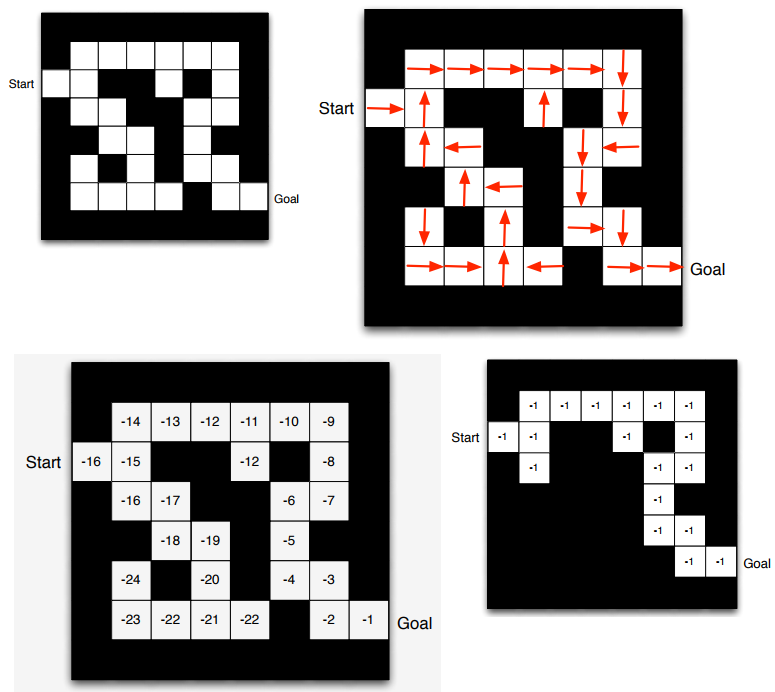
\includegraphics[width=\textwidth]{maze}
\caption{Upper left: Maze example. Upper right: Policy for maze. Lower left: Value function for maze. Lower right: Reward prediction for maze.}
\label{fig:maze}
\end{figure}

\subsection{Example: Maze}
As an example, consider an agent that has to find its way though the maze in the upper left of figure \ref{fig:maze}.  The problem has the following qualities:
\begin{itemize}
\item Rewards: We want the agent to get through the maze as quickly as possible, so each time step has a reward of -1.
\item Actions: The agent can move up, down, left, or right in each time step.
\item State: The state is the agents current position square in the maze.
\end{itemize}

A good policy for solving the problem is shown in the upper right. Here the arrows dictates the action given the state (position).

The lower left shows the value function corresponding to the policy: The future reward is negative the number of steps needed to get out of the maze from the current state (position). An optimal action can be chosen greedily, by picking the possibility with the lowest value of the function.

The lower right shows a reward prediction model for the maze. This one technically depends on both state and action, but as we no it is -1 no matter what.

\subsection{Categorization of agents}
Based on the above, we can broadly categorize agents into several categories:
\begin{itemize}
\item\textit{Value based agents} are based on a value function - with the policy being implicit. I.e. in each step we can greedily pick the action with the highest future reward, based directly on the value function.
\item\textit{Policy based agents} on the other hand has the policy as its key ingredient. Here, the policy mapping directly shows what action to take in each state.
\item\textit{Actor critic agents} takes both a poicy and a value function into account. Ideally the "best of both worlds".
\item\textit{Model free agents} may by policy and/or value function based, but has no model! I.e. it doesn't try to make predictions about the environment.
\item\textit{Model agents} may by policy and/or value function based, but includes modelling.
\end{itemize}

\section{Reinforcement learning and planning}
There's two fundamental types of problems in sequential decision making: \textit{Reinforcement learning} and \textit{planning}.

Reinforcement learning can be viewed as dumping the agent into an alien environment it initially knows nothing about. The agent then begins to interact with the environment, eventually improving its policy for doing so.

Planning is the situation where the agent starts with a perfect model of the environment. The agent then uses this model to make calculations without any external interaction, which then informs policy.

So in planning, we can in principle look many steps ahead, determining states and rewards (or expectation values thereof) and use this to pick optimal actions. In other words, a tree search.

\subsection{Exploration versus exploitation}
So reinforcement learning is very much a trial-and-error process. The agent should hopefully learn an effective policy from interacting with the environment. This requires \textit{exploration}. Ideally without losing too much reward along the way.

\begin{quotation}
Exploration finds more information about the environment.
\end{quotation}

Planning, on the other hand relies on \textit{exploitation} of the complete knowledge of the environment.

\begin{quotation}
Exploitation uses known information to maximize reward.
\end{quotation}

Usually, a combination of exploration and exploitation is necessary for achieving success. So there's a balance between the two, sometimes knows as \textit{exploration-exploitation tradeoff}. This consideration is unique to reinforcement learning as opposed to machine learning as a whole.

\subsubsection{Examples}
Situation: You're going out to eat.
\begin{itemize}
\item Exploitation: Going to your favorite restaurant.
\item Exploration: Trying a new restaurant.
\end{itemize}
Situation: Online banner advertisement.
\begin{itemize}
\item Exploitation: Show the most succesful advert so far.
\item Exploration: Display a different advert.
\end{itemize}
Situation: Drilling for oil.
\begin{itemize}
\item Exploitation: Drill at the best known location.
\item Exploration: Drill at a new location.
\end{itemize}

\subsection{Prediction and control}
\textit{Prediction} is trying out a given policy in practice and evaluating the results.

\textit{Control} on the other hand is optimizing the future, i.e. finding the best strategy.

Usually in reinforcement learning, we have to do prediction in order to control.

\section{Markov decision processes}
Recall that a Markov decision process (or MDP for short) is a case where everything about the environment is known - the agent state is the same as the environment state. This also means that it has the Markov property.

It turns out that almost all reinforcement learning problems can be restated as MDP's. For instance:
\begin{itemize}
\item Optimal control primarily deals with continuous MDP's.
\item Partially observable problems can be conversted into MDP's.
\item \textit{Bandits} are MDP's with one state.
\end{itemize}

\subsection{Transition probability matrix}
Consider for a moment an agent with a state having the Markov property, which simply takes the same (or no) action in every time step. Then given the initial state $s$ there is a probability it will end up in state $s'$ in the next time step - it can depend only on $s$ and $s'$ per the Markov property:
\begin{equation}
\mathcal{P}_{ss'}=\mathbb{P}[S_{t+1}=s'|S_t=s]
\end{equation}
These propabilities form a matrix; the \textit{transition probability matrix} $\mathcal{P}$:
\begin{equation}
\mathcal{P}=\begin{pmatrix}
\mathcal{P}_{11} & \mathcal{P}_{12} & \cdots & \mathcal{P}_{1n}\\
\mathcal{P}_{21} & \mathcal{P}_{22} & \cdots & \mathcal{P}_{2n}\\
\vdots & \vdots & \ddots & \vdots \\
\mathcal{P}_{n1} & \mathcal{P}_{n2} & \cdots & \mathcal{P}_{nn}
\end{pmatrix}
\end{equation}
This form assumes a finite number of states $n$, but in principle this can be infinite.

Because the entries are probabilites, each row of $\mathbb{P}$ must sum to 1:
\begin{equation}
\forall i\in\{1, 2,\ldots,n\}:\ \sum_{j=1}^n\mathcal{P}_{ij}=1
\end{equation}

Such a system - represented by the tuple $\langle S,\mathcal{P}\rangle$ - is known as a \textit{Markov process} or \textit{Markov chain}.

\subsection{Markov reward processes}
A \textit{Markov reward process} (or MRP) is a Markov process with a finite set of states and a \textit{reward function} $\mathcal{R}$ as well as a discount factor $\gamma\in[0,1]$. The reward function is defined as the expectation value of the next reward given the current state:
\begin{equation}
\mathcal{R}: s\mapsto\mathcal{R}_s=\mathbb{E}[R_{t+1}|S_t=s]
\label{reward}
\end{equation}
So a Markov reward process is the tuple $\langle S,\mathcal{P},\mathcal{R},\gamma\rangle$

\subsection{Return and value function}
The \textit{return} of a given outcome of a Markov reward process\footnote{Or of any system with rewards and a discounting factor $\gamma$, really.} is:
\begin{equation}
G_t=R_{t+1}+\gamma R_{t+2}+\gamma^2 R_{t+3}+\cdots=\sum_{n=1}^\infty \gamma^{n-1} R_{t+n}
\label{return}
\end{equation}
In other words, the return is the discounted future reward. This is the quantity we wish to maximize.

The value function, as we've already discussed above, is the expectation value of the return:
\begin{equation}
v(s)=\mathbb{E}[G_t|S_t=s]
\label{value}
\end{equation}

\subsection{The Bellman equation for MRP's}
We can now use equations \ref{value}, \ref{return}, and \ref{reward} to get a recursive formula for the value function:
\begin{align}
v(s)=&\mathbb{E}[G_t|S_t=s]=\\
&\mathbb{E}[R_{t+1}+\gamma R_{t+2}+\gamma^2 R_{t+3}+\cdots|S_t=s]=\\
&\mathbb{E}[R_{t+1}+\gamma(R_{t+2}+\gamma R_{t+3}+\gamma^2 R_{t+4}+\cdots)|S=s]=\\
&\mathbb{E}[R_{t+1}+\gamma G_{t+1}|S_t=s]=\\
&\mathbb{E}[R_{t+1}|S_t=s]+\gamma\mathbb{E}[G_{t+1}|S_t=s]=\\
&\mathcal{R}_s+\gamma\sum_{s'=1}^n\mathbb{P}[G_{t+1}|S_{t+1}=s']\mathbb{P}[S_{t+1}=s']=\\
&\mathcal{R}_s+\gamma\sum_{s'=1}^n\mathcal{P}_{ss'}v(s')
\end{align}
Summing it up:
\begin{equation}
v(s)=\mathcal{R}_s+\gamma\sum_{s'=1}^n\mathcal{P}_{ss'}v(s')
\label{bellman}
\end{equation}
Treating the value and reward functions as vectors $v$ and $\mathcal{R}$, this can be rewritten in matrix form:
\begin{equation}
v=\mathcal{R}+\gamma\mathcal{P}v
\label{belmann_matrix}
\end{equation} 

\end{document}